%! TEX program = xelatex
\documentclass[tikz]{standalone}
\usepackage[lining]{ebgaramond}
\usepackage[math-style=ISO, bold-style=ISO]{unicode-math}
\setmathfont{Garamond-Math.otf}
\begin{document}
  \begin{tikzpicture}[scale=1, transform shape]
    \node at ( 0.0,-1.4) {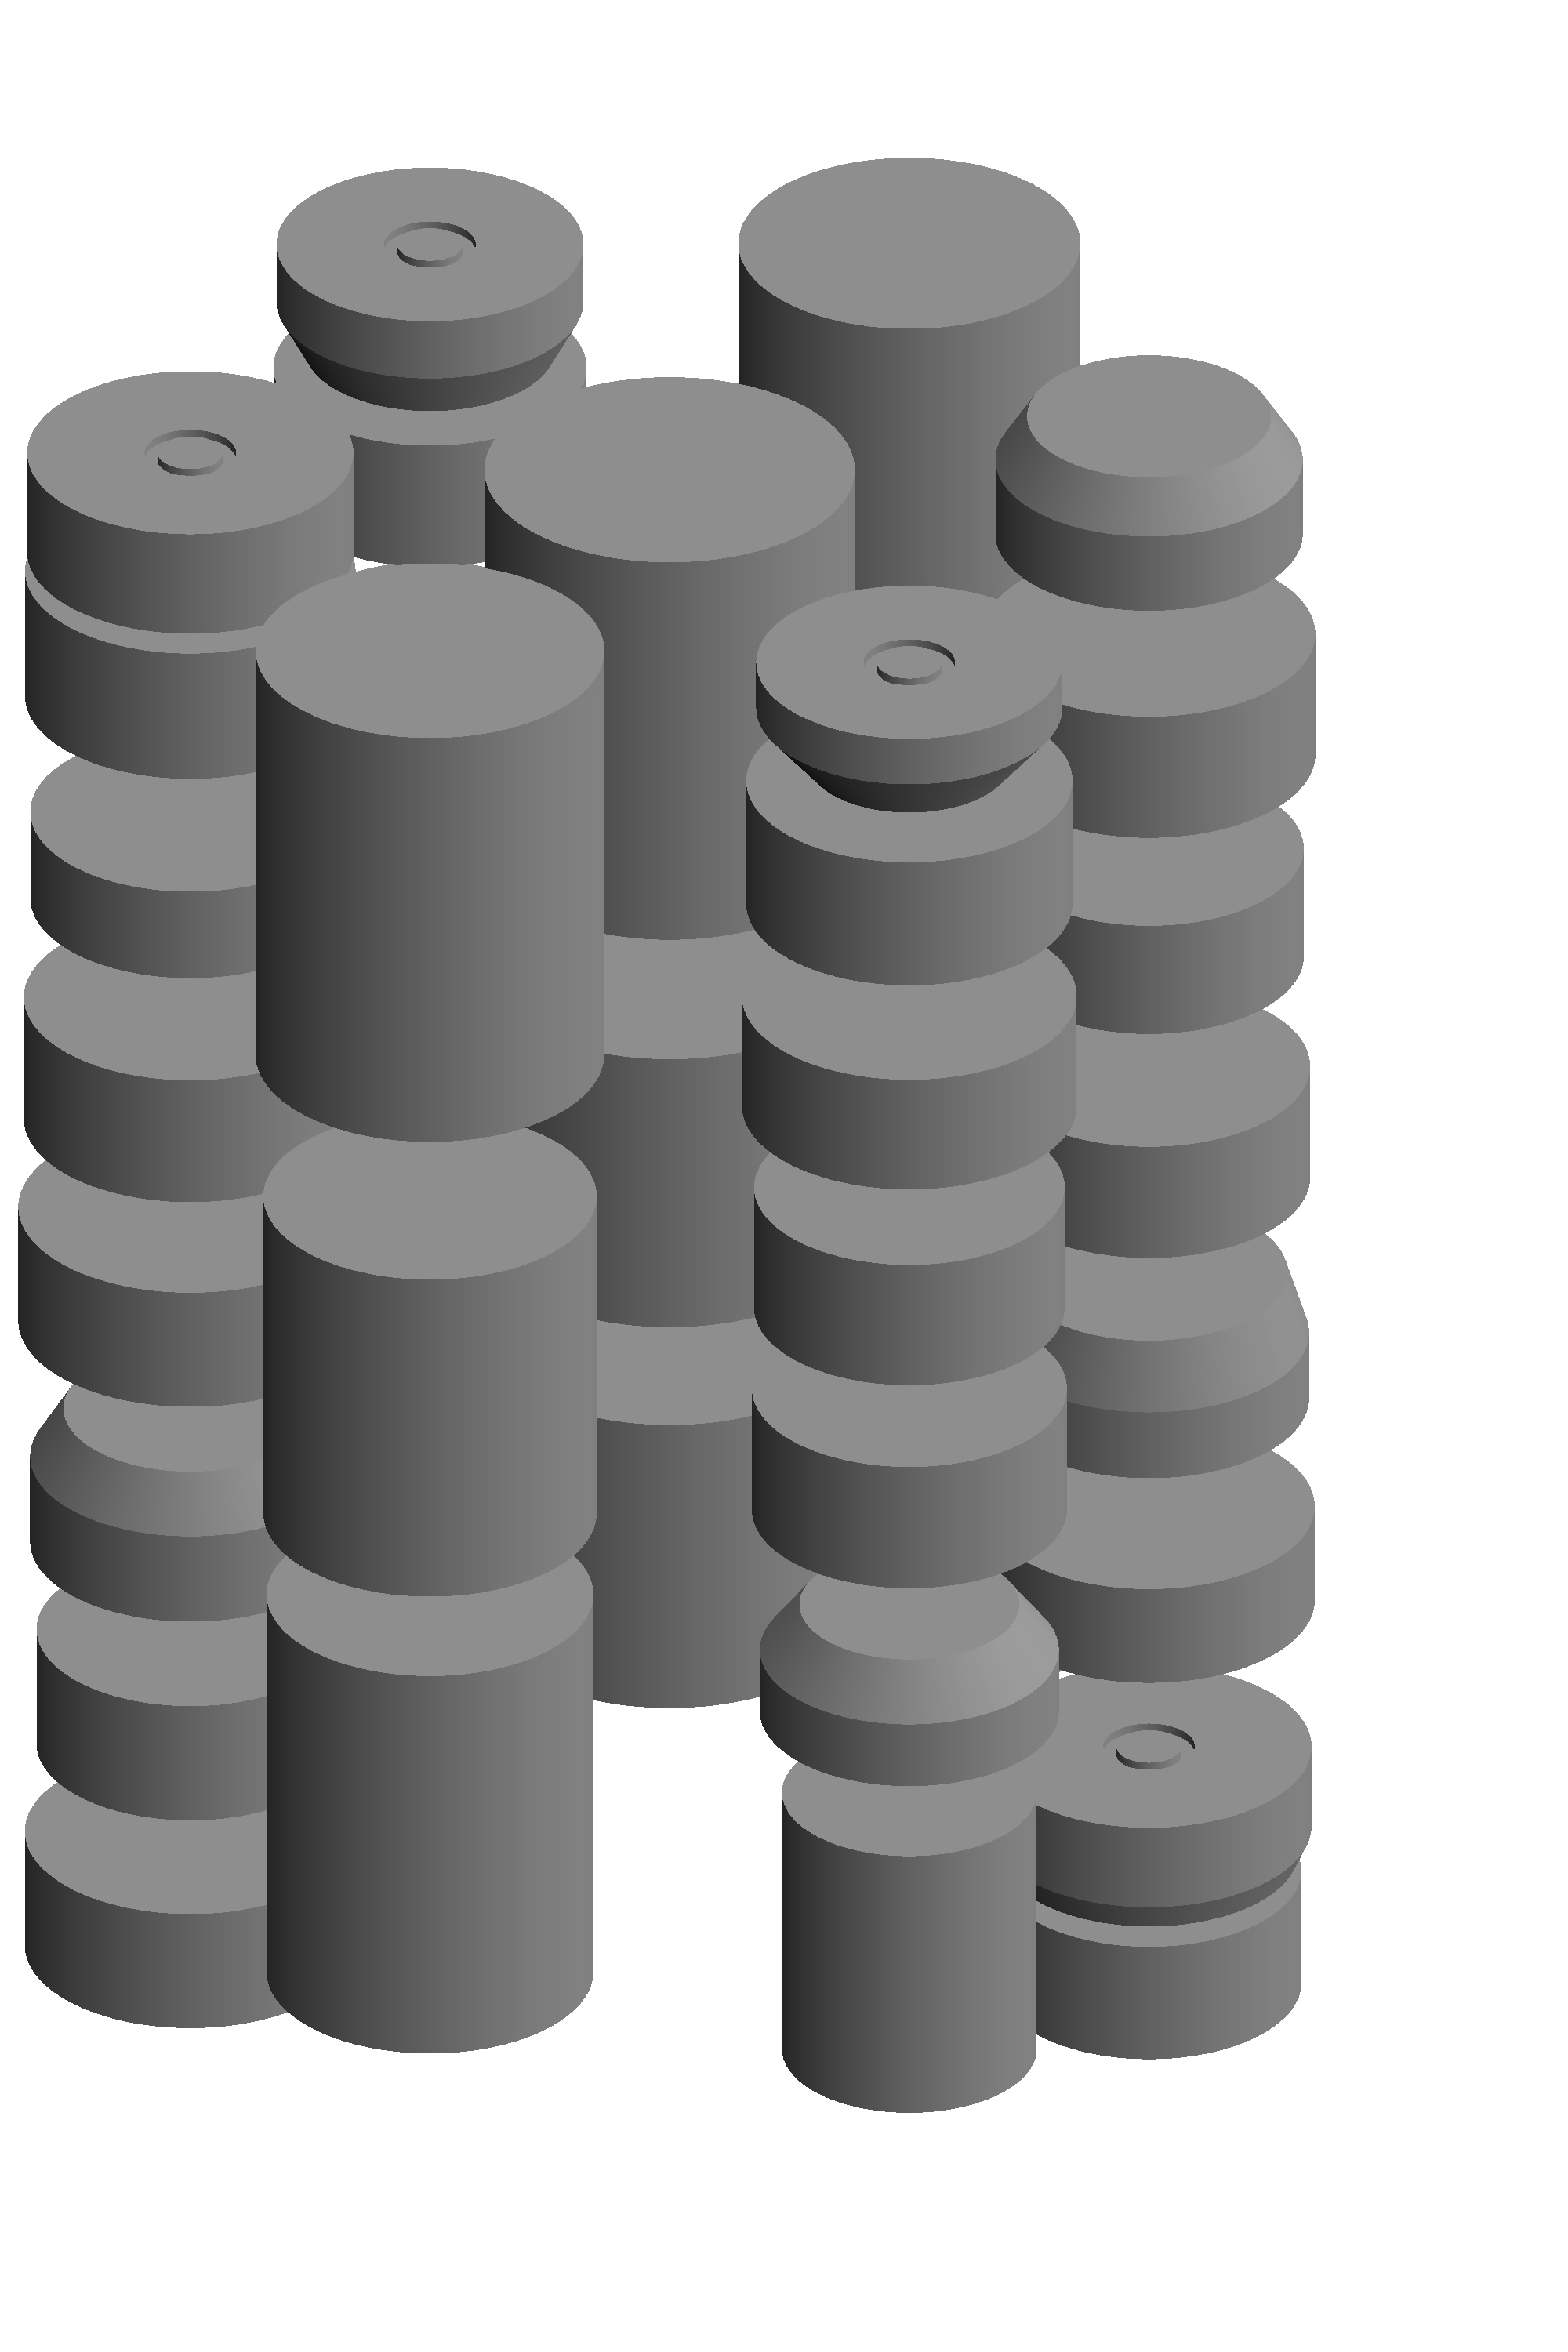
\includegraphics[height=4cm]{mage/diodes.jpeg}};
    \node at ( 2.6,-0.7) {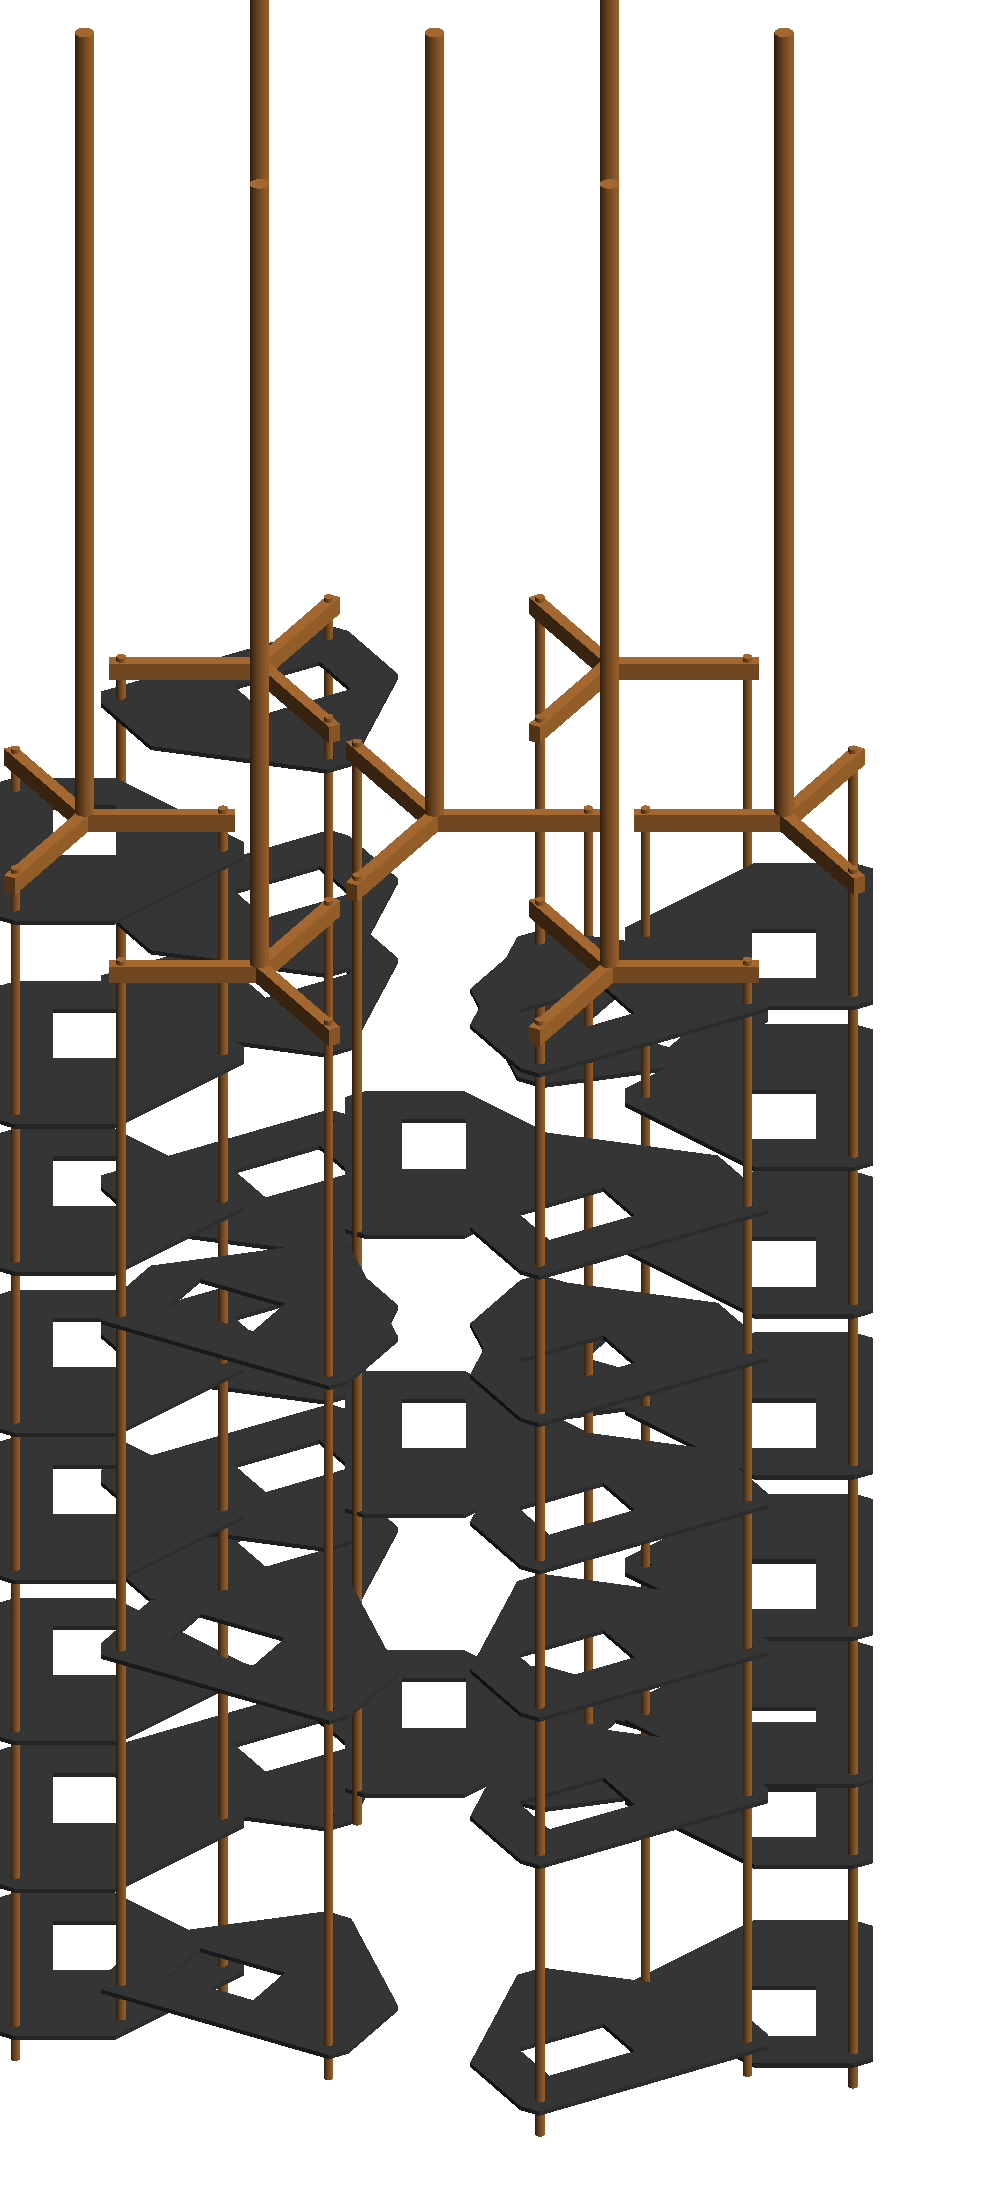
\includegraphics[height=5cm]{mage/holders.jpeg}};
    \node at ( 5.0, 0.1) {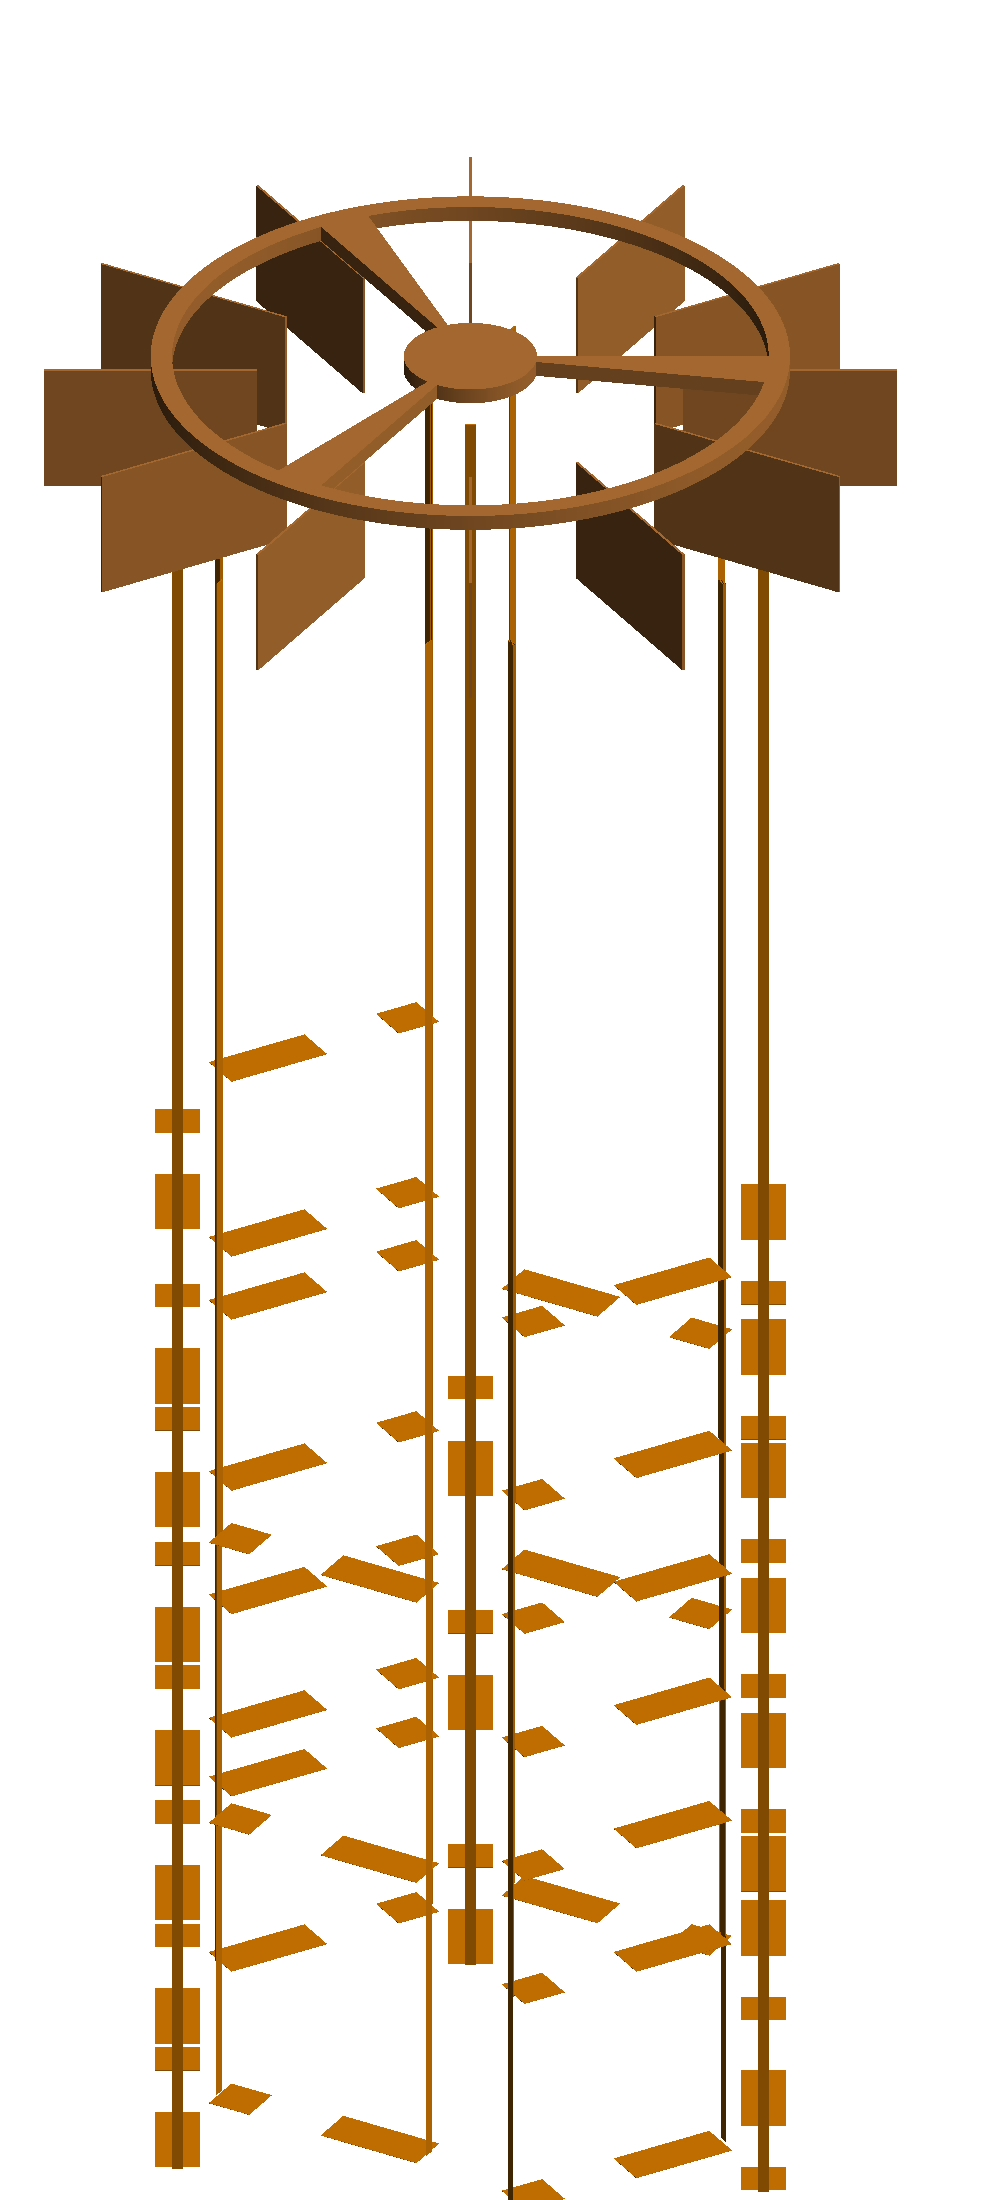
\includegraphics[height=6cm]{mage/cables.jpeg}};
    \node at ( 7.6, 0.0) {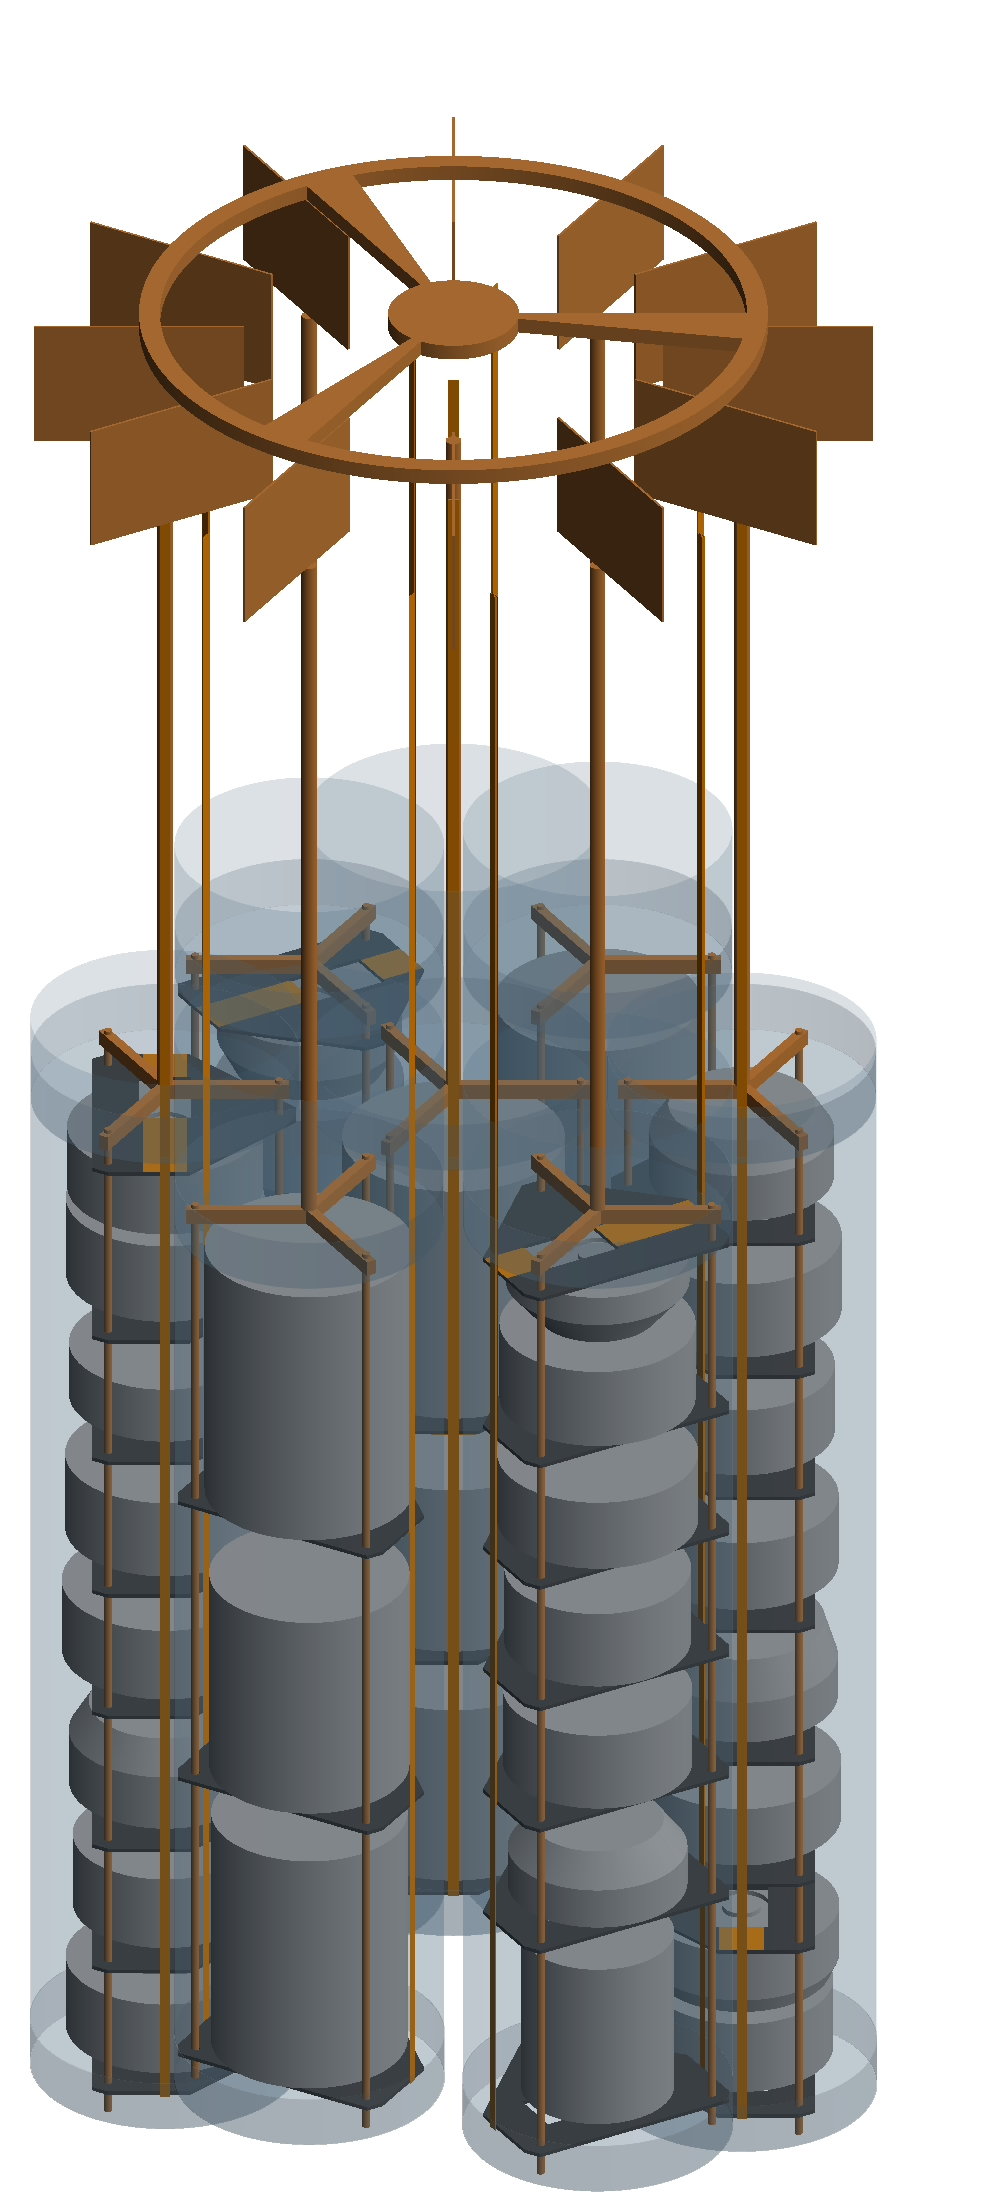
\includegraphics[height=6cm]{mage/full-array.jpeg}};
    \node at (10.0, 0.7) {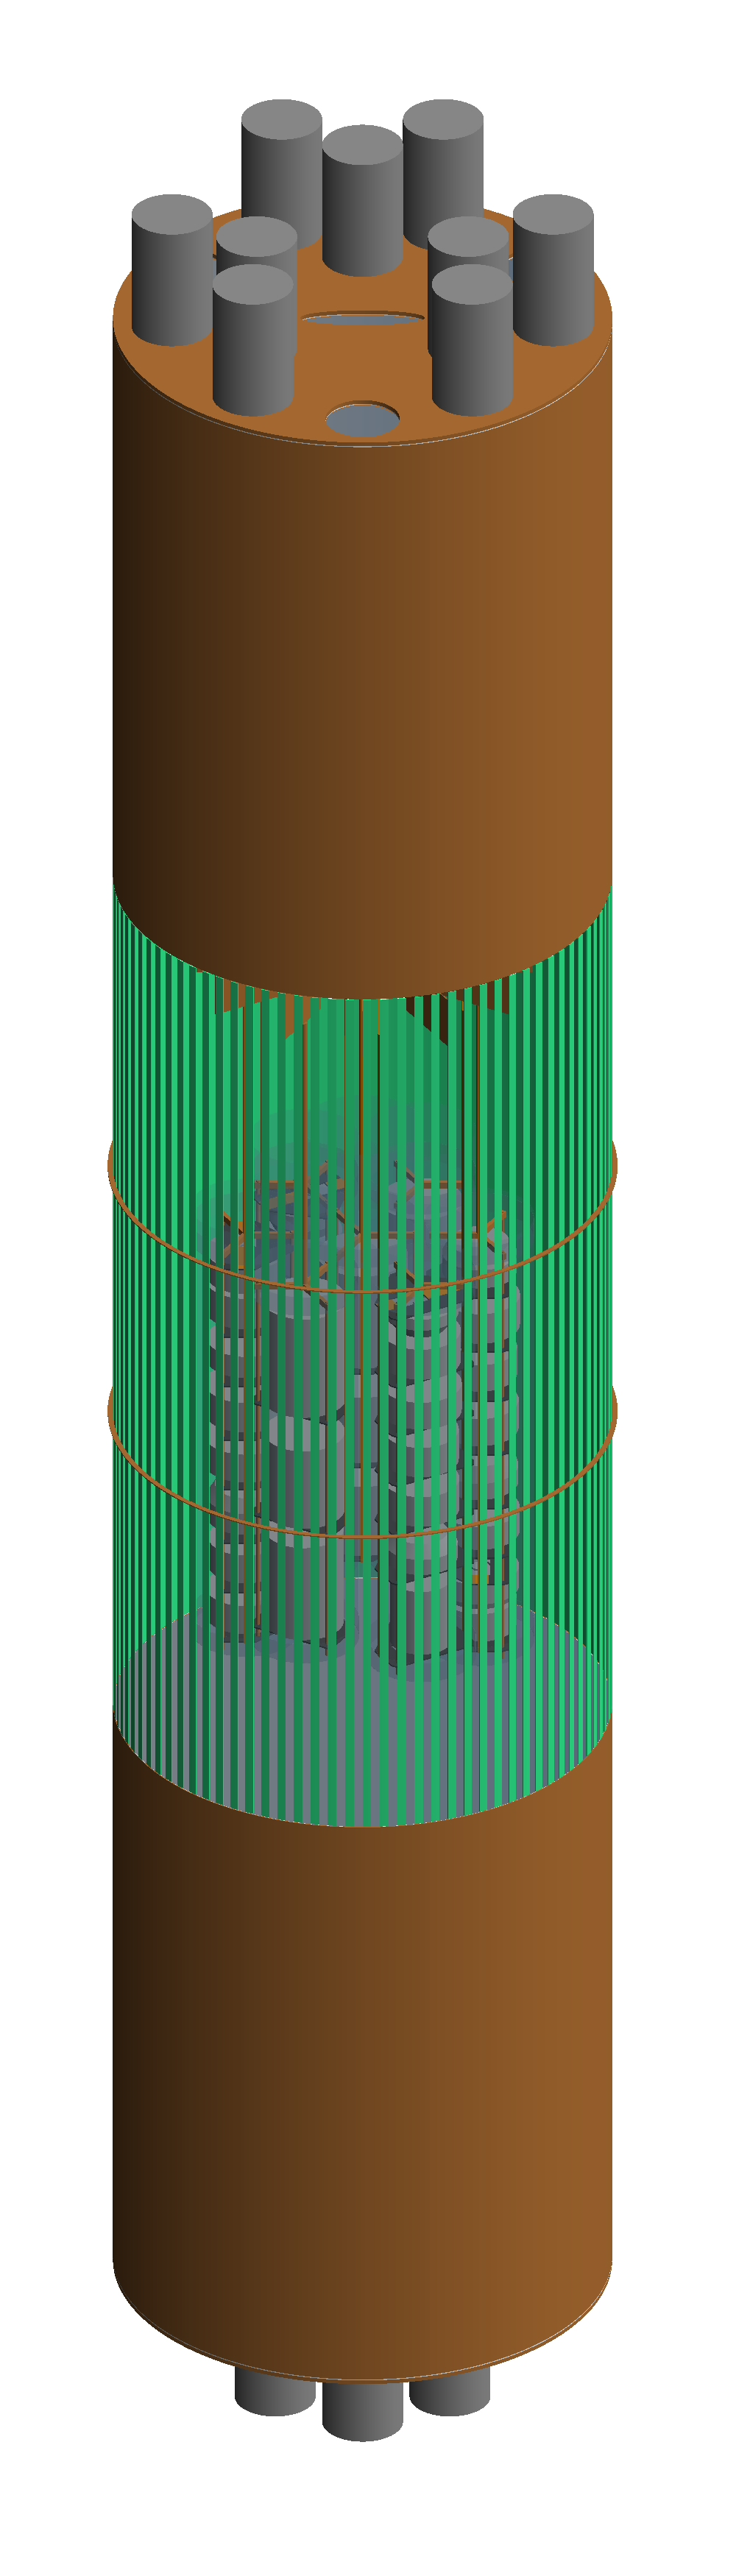
\includegraphics[height=8cm]{mage/full-larveto.jpeg}};
    \node at (12.2, 0.7) {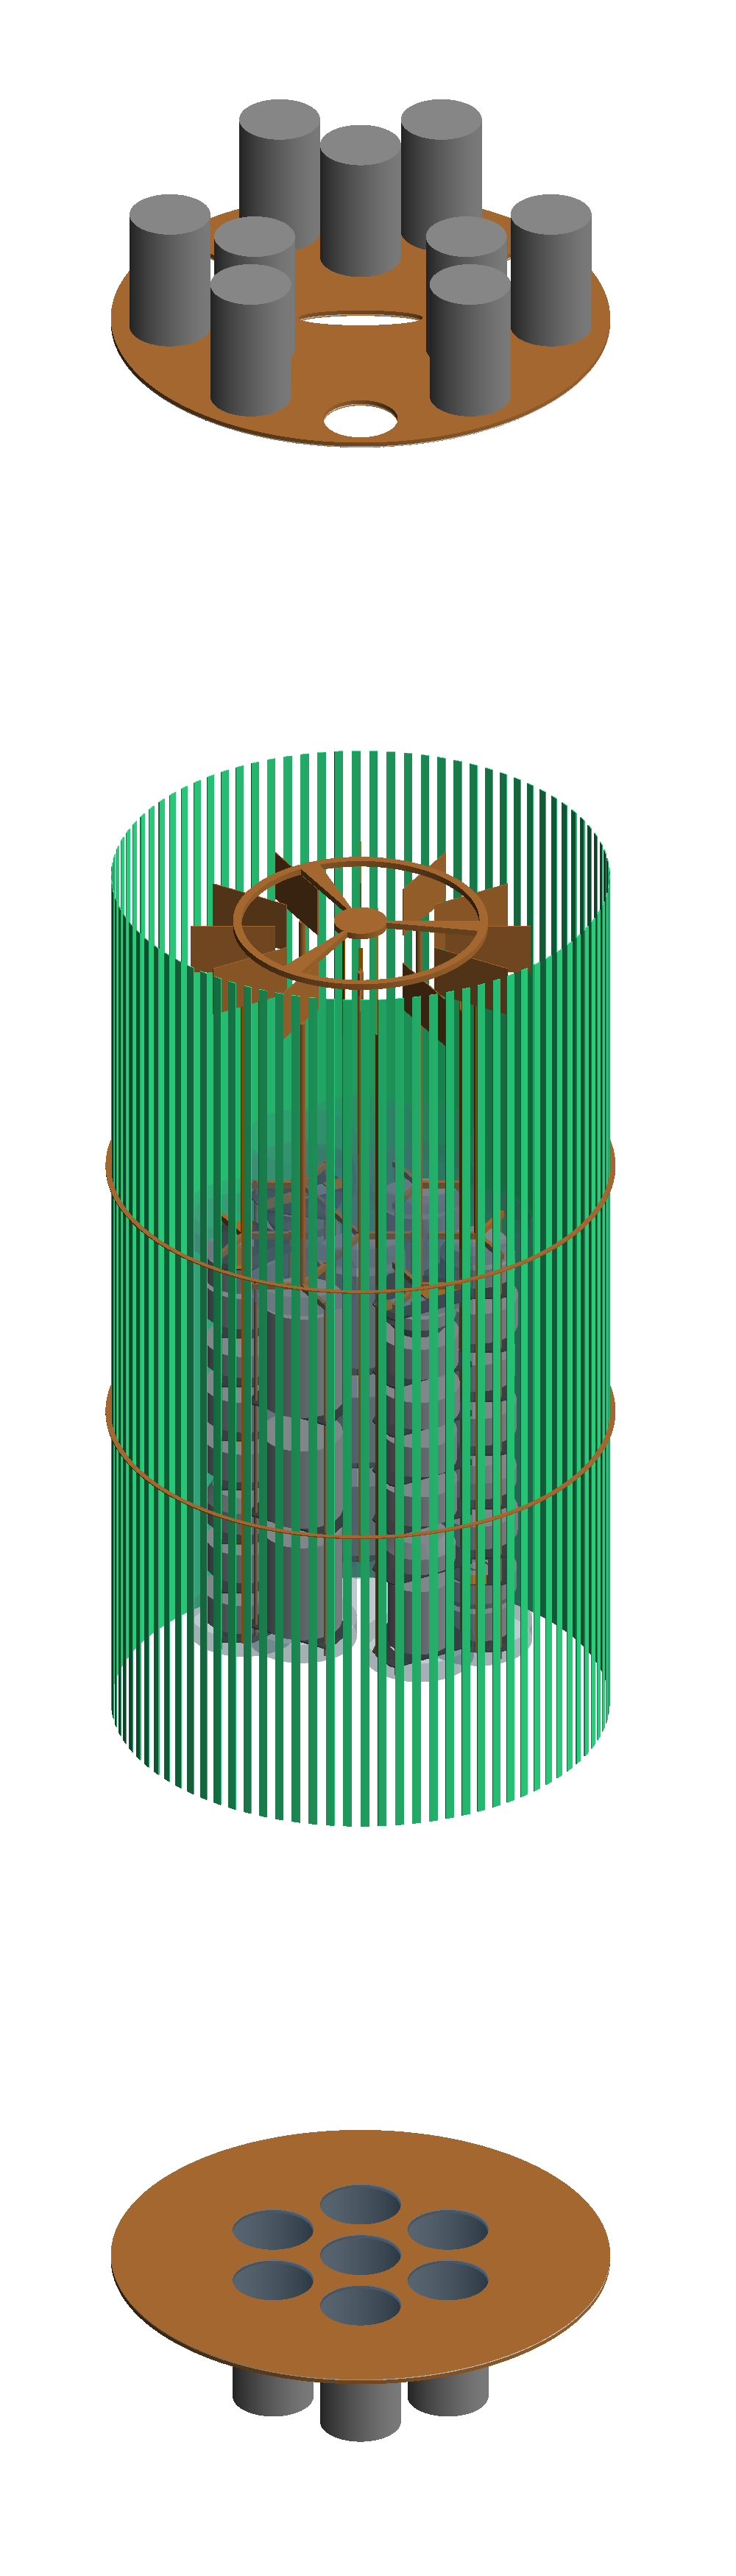
\includegraphics[height=8cm]{mage/larveto-noshroud.jpeg}};

    \node at (-0.2,-3.5) {(a)};
    \node at ( 2.5,-3.5) {(b)};
    \node at ( 4.9,-3.5) {(c)};
    \node at ( 7.5,-3.5) {(d)};
    \node at (10.0,-3.5) {(e)};
    \node at (12.2,-3.5) {(f)};
  \end{tikzpicture}
\end{document}
